\documentclass[12pt]{article}

\usepackage{mathtools}
\usepackage{blindtext}
% \usepackage{bbding}

% \usepackage[margin=1in]{geometry}

\newcommand*{\eu}{e}
\newcommand*{\iu}{i}

\DeclarePairedDelimiter{\bra}{\langle}{\rvert}
\DeclarePairedDelimiter{\ket}{\lvert}{\rangle}
\DeclarePairedDelimiterX{\braket}[2]{\langle}{\rangle}
  {#1\,\delimsize\vert\,\mathopen{}#2}

\usepackage{biblatex}
\addbibresource{report.bib}

\usepackage[hidelinks]{hyperref}

\title{Solving the Transverse-Field Ising Model on a Quantum Computer}
\author{David Basoco \and Jack Hetherington \and Davis Rash \and Tim Ross}
\date{October 4, 2023}

\begin{document}
  \maketitle

  \section{Introduction}
  The transverse-field Ising model is a quantum mechanical model of lattice sites with spin. In one dimension, the model can be described by the Hamiltonian
  \begin{equation}
    \label{eq:hamiltonian}
    H = \sum_{i = 1}^{n} \sigma_{i}^{x} \sigma_{i + 1}^{x}
        + \sigma_{1}^{y} \sigma_{2}^{z} \dotsm \sigma_{n - 1}^{z} \sigma_{n}^{y}
        + \lambda \sum_{i = 1}^{n} \sigma_{i}^{z},
  \end{equation}
  where \( \lambda \) is the transverse magnetic field strength. The second term maps periodic boundary conditions to fermionic degrees of freedom. Its effect vanishes for \( n \to \infty \) but will alter our result for \( n = 4 \).

  We simulated the Ising model on quantum simulators and the \texttt{ibm\_nairobi} 7-qubit quantum computer for \( n = 4 \) and compare our results to the original findings~\cite{Cervera18}.

  \section{Quantum Gate Operations}
  To solve Eq.~\eqref{eq:hamiltonian} on a quantum computer, we first

  To accurately decompose the Ising model Hamiltonian we need to take a decoupled Hamiltonian and convert it to the Ising model Hamiltonian. We can obtain this by applying a unitary disentangling operator such that
  \begin{equation}
    \tilde{H}
      = U_{\textnormal{dis}}^{\dagger} H
        U_{\textnormal{dis}}^{\vphantom{\dagger}},
  \end{equation}
  where \( H \) is the model Hamiltonian and \( \tilde{H} \) is a non interacting Hamiltonian. For the case of the Ising Hamiltonian, the method to obtain the \( U_{\textnormal{dis}} \) is threefold.
  \begin{enumerate}
   \item We first need to map spins to fermionic modes with the Jordan--Wigner transform.
   \item Then we need to get the fermions in moment space by applying the Quantum Fourier transform.
   \item Finally, we perform the Bogoliubov transform to decouple the modes in opposite momenta.
  \end{enumerate}
  This gives us the three-step recipe for out unitary disentangling operator:
  \begin{equation}
    U_{\textnormal{dis}}
      = U_{\textnormal{JW}} U_{\textnormal{FT}} U_{\textnormal{Bog}}
  \end{equation}

  \subsection{Jordan--Wigner Transform}
  The Jordan--Wigner transformation converts spin operators into the fermionic creation and annihilation operators.

  Under the Jodan--Wigner transformation
  \begin{align}
    \label{eq:jordan-wigner}
    c_{j}
      &= \biggl( \prod_{l < j} \sigma_{l}^{z} \biggr)
         \frac{\sigma_{j}^{x} - \iu \sigma_{j}^{y}}{2},
    &
    c_{j}^{\dagger}
      &= \frac{\sigma^{x}_{j} - \iu \sigma^{y}_{j}}{2}
         \biggl( \prod_{l < j} \sigma^{z}_{l} \biggr),
  \end{align}

  Then the Hamiltonian becomes
  \begin{equation}
    \label{eq:hamiltonian-fermion}
    H_{c}
      = \frac{1}{2}
        \sum_{i = 1}^{n} (c_{i + 1}^{\dagger} c_{i}^{\vphantom{\dagger}}
                          + c_{i}^{\dagger} c_{i + 1}^{\vphantom{\dagger}}
                          + c_{i}^{\dagger} c_{i + 1}^{\dagger}
                          + c_{i}^{\vphantom{\dagger}}
                            c_{i + 1}^{\vphantom{\dagger}})
        + \lambda \sum_{i = 1}^{n} c_{i}^{\dagger} c_{i}^{\vphantom{\dagger}}.
  \end{equation}
  Fortunately, the Jordan--Wigner transformation requires no gates to implement; it is a simple relabeling of the qubits. However, now any swapping must be done with the fermionic SWAP (fSWAP) gate
  \begin{equation}
    \label{eq:fswap}
    \mathrm{fSWAP}
      = \begin{pmatrix}
          1 & 0 & 0 & 0 \\
          0 & 0 & 1 & 0 \\
          0 & 1 & 0 & 0 \\
          0 & 0 & 0 & -1
        \end{pmatrix}.
  \end{equation}

  \subsection{Quantum Fourier Transform}
  Now we need to get the fermionic modes to momentum space with the quantum Fourier Transform.

  \begin{equation}
    \label{eq:qft}
    b_{k}
      = \frac{1}{\sqrt{n}}
        \sum_{j = 1}^{n} \eu^{2 \pi \iu j k / n} c_{j}, \qquad
    k = -\frac{n}{2} + 1, \dotsc, \frac{n}{2}
  \end{equation}

  Although this is valid in general, we have \( n = 2^{m} \), permitting us to use the fast Fourier transform.

  \subsection{Bogoliubov Transform}
  The final step is to decouple the modes that have opposite momentum. This will act over two qubit gates that represent opposite momenta.
  \begin{equation}
    B_{k}^{n}
      = \begin{pmatrix}
              \cos(\theta_{k} / n) & 0 & 0 & \iu \sin(\theta_{k} / n) \\
                                 0 & 1 & 0 &                        0 \\
                                 0 & 0 & 1 &                        0 \\
          \iu \sin(\theta_{k} / n) & 0 & 0 &     \cos(\theta_{k} / n)
      \end{pmatrix},
  \end{equation}
  \begin{equation}
    \theta_{k}
      = \arccos
        \frac{\lambda - \cos(2 \pi k / n)}
             {\sqrt{(\lambda - \cos(2 \pi k / n))^{2} + \sin^{2}(2 \pi k / n)}}.
  \end{equation}
  This returns our diagonal Hamiltonian
    \begin{equation}
      \tilde{H}
        = H_{a}
        = \sum_{k = -n / 2 + 1}^{n / 2}
          \omega_{k}^{\vphantom{\dagger}} a_{k}^{\dagger}
          a_{k}^{\vphantom{\dagger}},
    \end{equation}
    where
    \begin{equation}
      \omega_{k}
        = \sqrt{\biggl( \lambda - \cos \frac{2\pi k}{n} \biggr)^{2}
                + \sin^{2} \frac{2\pi k}{n}}.
    \end{equation}
    This result is consistant with a transformation which mixes the two modes in accordance with
    \begin{subequations}
      \begin{align}
        a_{k}
          &= u_{k}^{\vphantom{\dagger}} b_{k}^{\vphantom{\dagger}}
             + \iu v_{k}^{\vphantom{\dagger}} b_{-k}^{\dagger}, \\
        a_{k}^{\dagger}
          &= u_{k}^{\vphantom{\dagger}} b_{k}^{\dagger}
             + \iu v_{k}^{\vphantom{\dagger}} b_{-k}^{\vphantom{\dagger}}.
      \end{align}
    \end{subequations}

  \section{Time Evolution}
  With $U_{dis}$ applied to the basis states we exactly time evolve the problem. The time evolution for a given state using the time-independent Hamiltonian is described using the time evolution unitary $U(t) \coloneqq \eu^{-itH}$:
  \begin{equation}
    \ket{\psi(t)} = U(t)\ket{\psi_{0}} = \sum_{i} \eu^{-it\epsilon_{i}} \ket{E_{i}}\braket{E_{i}}{\psi_{0}},
  \end{equation}
  where $\bra{\psi_{0}}$ is the initial state and $\epsilon_{i}$ are the corresponding energies of the Hamiltonian states $\ket{E_{i}}$. If the observable, M, is such that $[H,M] \neq 0$, then the expectation value of M, will show an oscillation in time given by
  \begin{equation}
    \left\langle M(t)\right\rangle = \sum_{i,j}\eu^{-it(\epsilon_{i}-\epsilon_{j})}\braket{\psi_{0}}{E_{j}}\bra{E_{j}}M\ket{E_{i}}\braket{E_{i}}{\psi_{0}}.
  \end{equation}
  We now have computational basis states from the eigenstates of the non-interacting Hamiltonian $\tilde{H}$ and all energies $\epsilon_{i}$. We can construct the time evolution for a given state $\ket{\psi_{0}}$ by expressing it in computational basis and adding the corresponding factors $\eu^{-it\epsilon_{i}}$. Given a 4 unit system, as example, we can express the wave function in the $\tilde{H}$ basis, using $U_{dis}^{\dagger}$, as
  \begin{equation}
    \ket{\psi_{0}} = U_{dis}^{\dagger}\ket{0000} = \cos \phi\ket{0000} + i\sin \phi\ket{1100},
  \end{equation}
  where $\phi = \arccos(\lambda/\sqrt{1+\lambda ^2})/2$. Then, we apply the time evolution operator to obtain $\ket{\psi (t)}$ on the computational basis $\ket{0000}$:

  \begin{equation}
    \ket{\psi (t)} = \biggl( \cos \phi\ket{00} + i\eu^{i4t\sqrt{1+\lambda ^2}} \sin \phi \ket{11} \biggr) \otimes \ket{00}
  \end{equation}
  This expression can be presented analytically,

  \begin{equation}
    \left\langle \sigma_{z} \right\rangle = \frac{1 + 2\lambda ^2 + \cos \biggl( 4t\sqrt{1 + \lambda ^2}\biggr)}{2 + 2\lambda ^2}.
  \end{equation}
  These steps are represented only briefly in the code but perform a the function to obtain the expectation value of transverse magnetization $M_{z} = \frac{1}{2}\left\langle \sigma_{z}\right\rangle$. We will now be able to test various magnetization factors, $\lambda$, in time to compare with each other. Assuming a sinusoidal result, factors to look for are frequency, amplitude, damping and starting value.

  \section{Results}
   
    \begin{figure}[h]
      \centering
      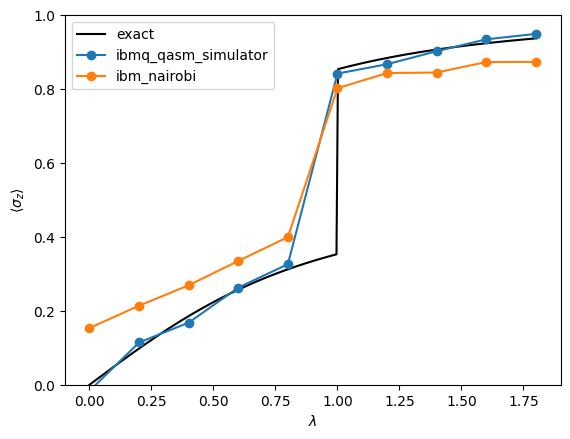
\includegraphics[width=0.7\textwidth]{images/ground-state-magnetization}
      \caption{The results obtained from running on both a quantum simulator and on a 7 qubit IBM quantum computer %
              \label{fig:ground-state-magnetization}}
    \end{figure}

    As seen in figure 1 both the simulated results and actual results are very close to the expected results. The differences on the real quantum computer are coming from the quantum noise present. The results also show an improvement over the Cervera-Lierta paper which showed a larger difference from the expected value for \begin{math}\lambda\end{math} greater than 1 than our results [1]. This could be due to improved quantum systems, which indicates that the Ising model could be used as a benchmark test for quantum computers. \\

    We had issues getting the time evolution section to run on the quantum computer, but the results from the simulator are presented below in figure 2.
    \begin{figure}[h!]
        \centering
        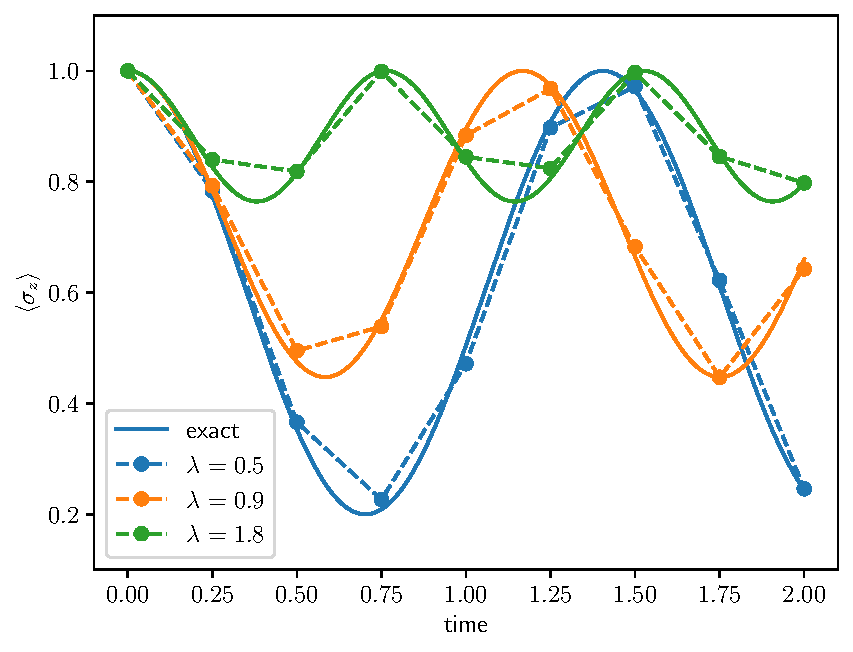
\includegraphics[width=0.7\textwidth]{images/time-evolution-magnetization-test}
        \caption{The time evolution results from ibmq-qasm-simulator %
              \label{fig:time-evolution-mangetization-test}}
    \end{figure}

    The simulated results match the expected results very closely, the only major differences are being caused by the sampling rate skipping over the relative minima and maxima for some of the simulations.

    \section{References}
    [1] Alba Cervera-Lierta. 2018. Exact Ising model simulation on a quantum computer.
Quantum (Dec. 2018). https://arxiv.org/pdf/1807.07112.pdf


\end{document}
